\section{Технический проект}
\subsection{Общая характеристика организации решения задачи}

Необходимо разработать веб-платформу, специально адаптированную для упрощения процесса обмена внутриигровыми ценностями в игре "Stay Out".

Веб-сайт представляет собой комплекс электронных страниц, объединенных в логическую структуру и содержащих разнообразную информацию, включая текст, графику и мультимедийные элементы. Этот онлайн-ресурс доступен через Интернет по определенному доменному имени, например, www.stayoutexchange.com. Каждая страница веб-сайта представляет собой HTML-документ, который обеспечивает визуальное и функциональное взаимодействие с пользователем при помощи языков программирования, таких как HTML, CSS и JavaScript.

Разрабатываемый веб-сайт будет предоставлять пользователям возможность создания учетных записей, выставления и поиска внутриигровых ценностей, а также обмена ими с другими игроками. Он будет обеспечивать удобный интерфейс для взаимодействия между игроками, обеспечивая прозрачность и безопасность сделок.

\subsection{Обоснование выбора технологии проектирования}

Используемые для создания программно-информационной системы языки и технологии отвечают современным практикам разработки, позволяют достичь высокой производительности и отказоустойчивости программы.

\subsubsection{Описание используемых технологий и языков программирования}

В процессе разработки web-сайта используются программные средства и языки программирования. Каждое программное средство и каждый язык программирования применяется для круга задач, при решении которых они необходимы.

\subsubsection{Язык программирования JavaScript}

JavaScript - это интерпретируемый, объектно-ориентированный язык программирования, который широко используется для создания интерактивных и динамических веб-сайтов. Благодаря своей многофункциональности, JavaScript является одним из самых популярных языков программирования в мире веб-разработки.

В отличие от многих других языков программирования, JavaScript выполняется непосредственно в web-браузере пользователя. Это позволяет ему взаимодействовать с элементами HTML страницы, управлять их содержимым, изменять стили, реагировать на пользовательские действия и многое другое, что делает веб-страницы более интерактивными и динамичными.

JavaScript широко используется для разработки различных веб-приложений, таких как интерфейсы пользователя, игры, анимации, формы обратной связи, веб-сервисы и многое другое. Благодаря своей популярности и гибкости, JavaScript также стал широко используемым для разработки серверной стороны приложений с использованием платформы Node.js.

Язык JavaScript имеет динамическую типизацию данных, что означает, что переменные не требуют явного объявления типа данных, и их тип может изменяться в процессе выполнения программы. Это делает JavaScript гибким и удобным для быстрой разработки прототипов и простых скриптов.

Важно отметить, что JavaScript не следует путать с языком Java, несмотря на сходство в названиях. JavaScript и Java - это разные языки программирования с разными синтаксисами, целями и областями применения. JavaScript был создан компанией Netscape в начале 1990-х годов и был изначально разработан для управления взаимодействием с пользователем на веб-страницах.

\paragraph{Достоинства языка JavaScript}

JavaScript чаще всего используется для написания сценариев работы с web-страницами в web-браузерах, обеспечивая программирование на стороне клиента. Этот язык предоставляет возможность доступа к элементам разметки web-страницы посредством объектов, что значительно упрощает манипуляции с разметкой. Для решения сложностей с интерпретацией кода различными браузерами применяется библиотека jQuery, которая расширяет возможности JavaScript и унифицирует поведение кода между разными средами.

\paragraph{Недостатки языка Javascript}

JavaScript обладает некоторыми особенностями, например, непредсказуемость операций сравнения типов данных, что может привести к неожиданным результатам при выполнении математических операций или сравнении значений. Это создает потенциальные сложности для разработчиков, так как различные web-браузеры могут по-разному интерпретировать сценарии JavaScript. Неверно написанный код JavaScript может привести к труднообнаруживаемым ошибкам, и их отладка может быть затруднительной из-за специфики языка.

\subsection{Диаграмма компонентов и схема обмена данными между файлами компонента}

Диаграмма компонентов является важным инструментом для описания физического представления разрабатываемой системы. Она позволяет разработчикам определить архитектуру системы, выявив взаимосвязи и зависимости между программными компонентами, включая как исходный, так и исполняемый код.

Основными элементами диаграммы компонентов являются компоненты, интерфейсы и зависимости между ними. Компоненты представляют собой логические единицы функциональности системы, которые могут быть как отдельными приложениями, так и более крупными модулями или сервисами.

Интерфейсы определяют способы взаимодействия между компонентами, задавая набор методов, сообщений или протоколов, которыми компоненты обмениваются информацией.

Зависимости указывают на связи между компонентами, определяя порядок и направление потока данных или контроля между ними.

На рисунке \ref{fig:comp} представлена диаграмма компонентов для проектируемой системы. В центре диаграммы находится сервер с операционной системой, на которой установлена система управления содержимым. Эта система включает в себя базу данных и интерфейс для взаимодействия с клиентскими приложениями.

Помимо этого на диаграмме изображен клиентский компьютер с операционной системой, на которой установлен браузер. Этот компьютер предоставляет интерфейс для взаимодействия пользователя с системой через web-интерфейс.

\vspace{-8mm}
\begin{figure}
	\centering
	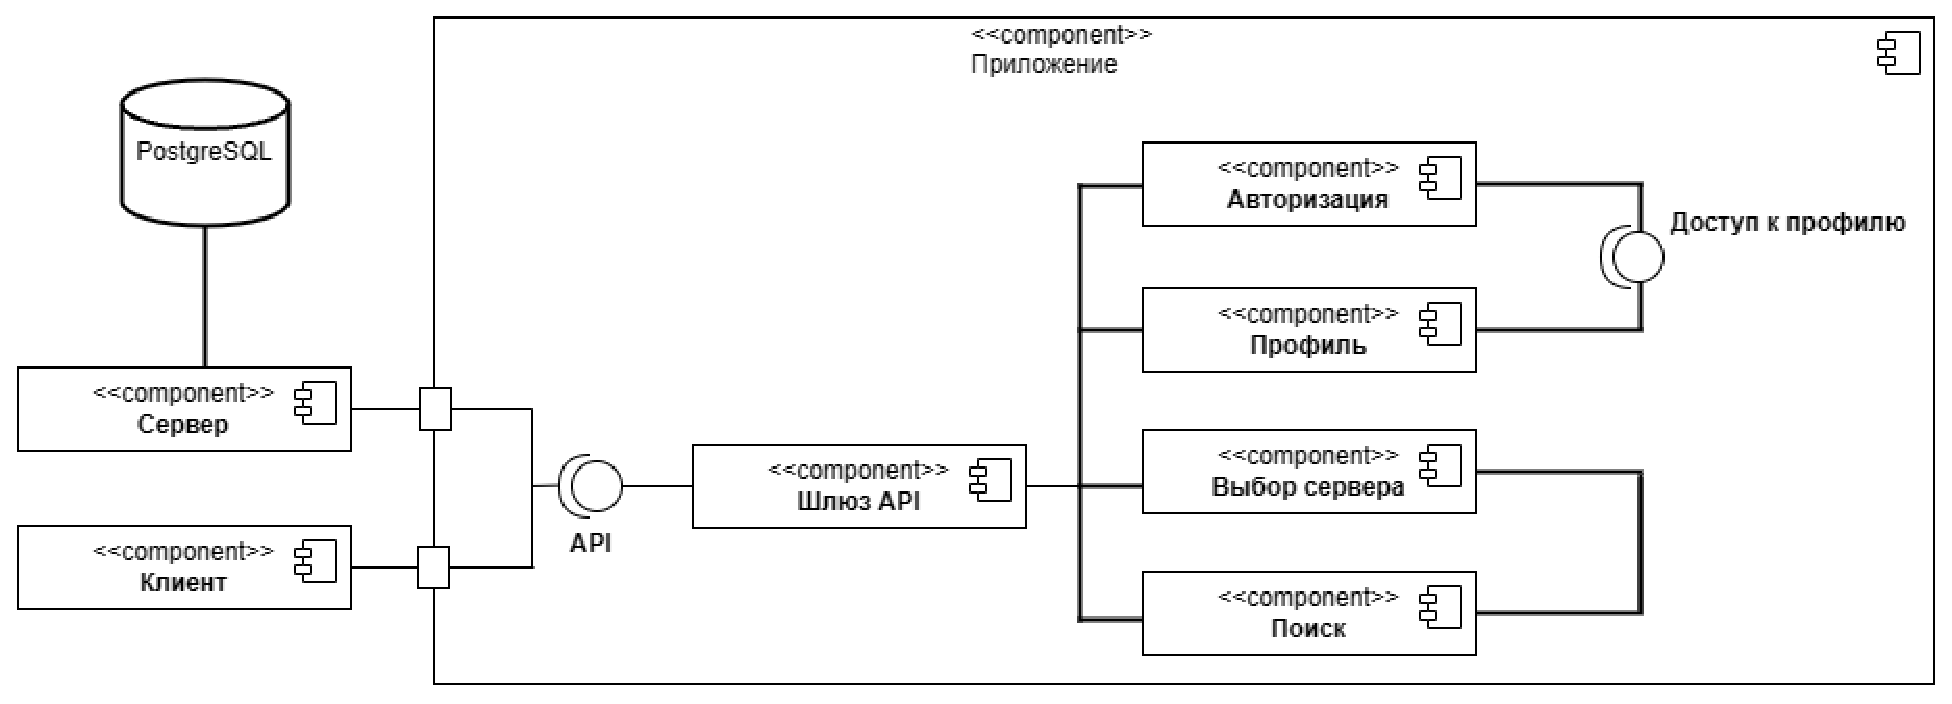
\includegraphics[width=1\linewidth]{images/comp}
	\caption{Диаграмма компонентов}
	\label{fig:comp}
\end{figure}

Любой компонент должен быть вызван в сценарии страницы web-сайта. Web-страница передает данные компоненту в момент вызова последнего.

При вызове компонента в сценарии web-страницы передаются значения параметров компонента, которые далее передаются в сценарий файла component.php через массив \$arParams.

В сценарии файла component.php происходит вызов одного из шаблонов компонента с помощью метода IncludeComponentTemplate класса CBitrixComponent. Id шаблона также определяется в сценарии страницы web-приложения и передается неявно методом IncludeComponentTemplate.

После вызова шаблона компонента, в файл template.php передается массив \$arParams, возможно, измененный в сценарии component.php, а также массив \$arResult, сформированный в самом сценарии component.php. Оба этих массива доступны также и в файле result\_modifier.php, который подключается перед template.php.

Работа компонента завершается после выполнения сценария файла component.php. Однако, если массив \$arResult будет изменен в сценарии шаблона, изменения не будут переданы обратно в сценарий файла компонента component.php.

\subsection{Диаграмма размещения}

Диаграмма размещения (рис.~\ref{fig:razm}) отражает физические взаимосвязи между программными и аппаратными компонентами системы.

\vspace{-8mm} % чтобы убрать пустую строку, которая осталась после переноса рисунка на следующую страницу
\begin{figure}
	\centering
	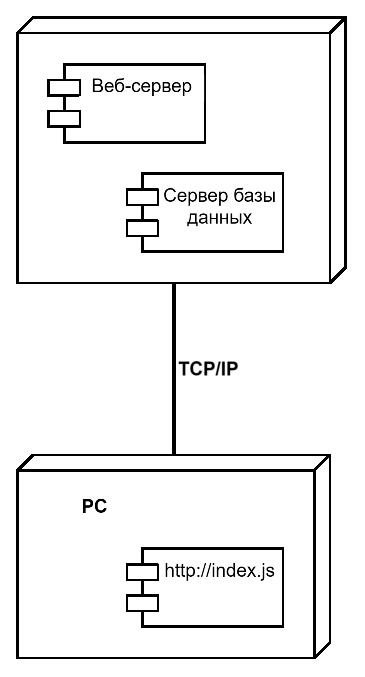
\includegraphics[width=0.5\linewidth]{images/razm}
	\caption{Диаграмма размещения}
	\label{fig:razm}
\end{figure}

Она является хорошим средством для показа маршрутов перемещения объектов и компонентов в распределенной системе.

В таблице \ref{ssevsws:table} приведен пример использования пакета xltabular с автоматическим расчетом ширины столбца.

\begin{xltabular}{\textwidth}{|c|X|X|}
	\caption{Сравнение протоколов SSE и WebSocket\label{ssevsws:table}}\\ \hline
	~  & \centrow  SSE & \centrow WebSocket \\ \hline
	\endfirsthead
	\continuecaption{Продолжение таблицы \ref{ssevsws:table}}
	~ & \centrow SSE & \centrow WebSocket \\ \hline 
	\finishhead
	Направленность & 
	Однонаправленный, полудуплексный: данные посылает только сервер & 
	Двунаправленный, полнодуплексный: и сервер, и клиент могут обмениваться сообщениями \\ \hline 
	Соединение  & HTTP & WS \\ \hline 
	Тип данных & Только текст & Бинарные и текстовые данные \\ \hline 
	Доп. возможности & Встроенный механизм идентификаторов событий и переподключения & Переподключение и идентификация события реализуются на стороне приложения
\end{xltabular}

\subsection{Содержание информационных блоков. Основные сущности}

Проанализировав требования, можно выделить шесть основных сущностей:
\begin{itemize}
\item "<Пользователь">;
\item "<Предметы">;
\item "<Услуги">.
\end{itemize}

В состав сущности "<Пользователь"> можно включить атрибуты, представленные в таблице \ref{news:table}.

\begin{xltabular}{\textwidth}{|l|l|p{1.7cm}|X|}
	\caption{Атрибуты сущности "<Пользователь">\label{news:table}}\\ \hline
	\centrow Поле & \centrow Тип & \centrow Обяза\-тельное & \centrow Описание \\ \hline
	\thead{1} & \thead{2} & \centrow 3 & \centrow 4 \\ \hline
	\endfirsthead
	\continuecaption{Продолжение таблицы \ref{news:table}}
	\thead{1} & \thead{2} & \centrow 3 & \centrow 4 \\ \hline
	\finishhead
	id & ObjectId & true & Уникальный идентификатор \\ \hline 
	email & String & true & Почта \\ \hline 
	login & String & true & Псевдоним \\ \hline
	password & String & true & Пароль \\ \hline 
	role & String & true & Привилегия \\ \hline 
	status & String & true & Статус \\ \hline 
\end{xltabular}

В состав сущности "<Предметы"> можно включить атрибуты, представленные в таблице \ref{proda:table}.

\begin{xltabular}{\textwidth}{|R|C{2.5cm}|l|T|}
	\caption{Атрибуты  сущности "<Предметы"> с использованием различных типов столбцов и многострочным заголовком\label{proda:table}}\\ \hline
	\centrow Поле & \centrow Тип & \centrow Обязательное & \centrow Описание \\ \hline
	\centrow 1 & \centrow 2 & \thead{3} & \centrow 4 \\ \hline
	\endfirsthead
	\continuecaption{Продолжение таблицы \ref{proda:table}}
	\centrow 1 & \centrow 2 & \thead{3} & \centrow 4 \\ \hline
	\finishhead
	id & ObjectId & true & Уникальный идентификатор \\ \hline 
	name & String & true & Название \\ \hline 
	description & String & false & Описание \\ \hline 
	img & String & true & Путь до изображения \\ \hline 
	weight & String & true & Вес \\ \hline 
	level & String & true & Уровень \\ \hline 
\end{xltabular}

В состав сущности "<Тип"> можно включить атрибуты, представленные в таблице \ref{prod1:table}.

\begin{xltabular}{\textwidth}{|R|C{2.5cm}|l|T|}
	\caption{Атрибуты  сущности "<Тип"> с использованием различных типов столбцов и многострочным заголовком\label{prod1:table}}\\ \hline
	\centrow Поле & \centrow Тип & \centrow Обязательное & \centrow Описание \\ \hline
	\centrow 1 & \centrow 2 & \thead{3} & \centrow 4 \\ \hline
	\endfirsthead
	\continuecaption{Продолжение таблицы \ref{prod1:table}}
	\centrow 1 & \centrow 2 & \thead{3} & \centrow 4 \\ \hline
	\finishhead
	id & ObjectId & true & Уникальный идентификатор \\ \hline 
	name & String & true & Название \\ \hline 
	img & String & true & Путь до изображения \\ \hline 
\end{xltabular}

В состав сущности "<Класс"> можно включить атрибуты, представленные в таблице \ref{prod2:table}.

\begin{xltabular}{\textwidth}{|R|C{2.5cm}|l|T|}
	\caption{Атрибуты  сущности "<Класс"> с использованием различных типов столбцов и многострочным заголовком\label{prod2:table}}\\ \hline
	\centrow Поле & \centrow Тип & \centrow Обязательное & \centrow Описание \\ \hline
	\centrow 1 & \centrow 2 & \thead{3} & \centrow 4 \\ \hline
	\endfirsthead
	\continuecaption{Продолжение таблицы \ref{prod2:table}}
	\centrow 1 & \centrow 2 & \thead{3} & \centrow 4 \\ \hline
	\finishhead
	id & ObjectId & true & Уникальный идентификатор \\ \hline 
	name & String & true & Название \\ \hline 
	img & String & true & Путь до изображения \\ \hline 
\end{xltabular}

В состав сущности "<Экипировка"> можно включить атрибуты, представленные в таблице \ref{prod3:table}.

\begin{xltabular}{\textwidth}{|R|C{2.5cm}|l|T|}
	\caption{Атрибуты  сущности "<Экипировка"> с использованием различных типов столбцов и многострочным заголовком\label{prod3:table}}\\ \hline
	\centrow Поле & \centrow Тип & \centrow Обязательное & \centrow Описание \\ \hline
	\centrow 1 & \centrow 2 & \thead{3} & \centrow 4 \\ \hline
	\endfirsthead
	\continuecaption{Продолжение таблицы \ref{prod3:table}}
	\centrow 1 & \centrow 2 & \thead{3} & \centrow 4 \\ \hline
	\finishhead
	id & ObjectId & true & Уникальный идентификатор \\ \hline 
	lifting\_capacity & String & true & Грузоподъемность \\ \hline 
	melee & String & true & Рукопашная \\ \hline 
	explosion & String & true & Взрыв \\ \hline
	electric & String & true & Электрическое \\ \hline 
	infrared & String & true & Инфракрасное \\ \hline 
	radiation & String & true & Радиация \\ \hline 
	biological & String & true & Биологическое \\ \hline 
	frostbite & String & true & Обморожение \\ \hline 
	state & String & true & Состояние \\ \hline 
\end{xltabular}

В состав сущности "<Патроны"> можно включить атрибуты, представленные в таблице \ref{prod4:table}.

\begin{xltabular}{\textwidth}{|R|C{2.5cm}|l|T|}
	\caption{Атрибуты  сущности "<Патроны"> с использованием различных типов столбцов и многострочным заголовком\label{prod4:table}}\\ \hline
	\centrow Поле & \centrow Тип & \centrow Обязательное & \centrow Описание \\ \hline
	\centrow 1 & \centrow 2 & \thead{3} & \centrow 4 \\ \hline
	\endfirsthead
	\continuecaption{Продолжение таблицы \ref{prod4:table}}
	\centrow 1 & \centrow 2 & \thead{3} & \centrow 4 \\ \hline
	\finishhead
	id & ObjectId & true & Уникальный идентификатор \\ \hline 
	type\_ammo & String & true & Тип \\ \hline 
	breaking\_throught & String & true & Пробитие \\ \hline 
	damage & String & true & Урон \\ \hline 
\end{xltabular}

В состав сущности "<Оружие"> можно включить атрибуты, представленные в таблице \ref{prod5:table}.

\begin{xltabular}{\textwidth}{|R|C{2.5cm}|l|T|}
	\caption{Атрибуты  сущности "<Оружие"> с использованием различных типов столбцов и многострочным заголовком\label{prod5:table}}\\ \hline
	\centrow Поле & \centrow Тип & \centrow Обязательное & \centrow Описание \\ \hline
	\centrow 1 & \centrow 2 & \thead{3} & \centrow 4 \\ \hline
	\endfirsthead
	\continuecaption{Продолжение таблицы \ref{prod5:table}}
	\centrow 1 & \centrow 2 & \thead{3} & \centrow 4 \\ \hline
	\finishhead
	id & ObjectId & true & Уникальный идентификатор \\ \hline 
	moa & String & true & Угловая минута \\ \hline 
	rate\_of\_fire & String & true & Темп \\ \hline 
	breaking\_throught & String & true & Пробитие \\ \hline 
	strength & String & true & Прочность \\ \hline 
	recoil & String & true & Отдача \\ \hline 
	handing & String & true & Качание \\ \hline 
	rocw & String & true & Отказ от состояния \\ \hline 
	no\_pollutin & String & true & Отказ от загрязнения \\ \hline 
	type\_ammo & String & true & Тип патрона \\ \hline 
\end{xltabular}

В состав сущности "<Гранаты"> можно включить атрибуты, представленные в таблице \ref{prod6:table}.

\begin{xltabular}{\textwidth}{|R|C{2.5cm}|l|T|}
	\caption{Атрибуты  сущности "<Гранаты"> с использованием различных типов столбцов и многострочным заголовком\label{prod6:table}}\\ \hline
	\centrow Поле & \centrow Тип & \centrow Обязательное & \centrow Описание \\ \hline
	\centrow 1 & \centrow 2 & \thead{3} & \centrow 4 \\ \hline
	\endfirsthead
	\continuecaption{Продолжение таблицы \ref{prod6:table}}
	\centrow 1 & \centrow 2 & \thead{3} & \centrow 4 \\ \hline
	\finishhead
	id & ObjectId & true & Уникальный идентификатор \\ \hline 
	number\_of\_fragments & String & true & Количество осколков \\ \hline 
	shock\_wave\_radius & String & true & Радиус взрыва \\ \hline 
\end{xltabular}

В системе предусмотрен внутренний механизм связи между разделами и элементами информационных блоков, что обеспечивает эффективную организацию данных без необходимости введения дополнительных идентификаторов при реализации связей между сущностями.

Каждая сущность в системе представлена экземпляром информационного блока, который содержит элементы, отражающие конкретные атрибуты или характеристики данной сущности. Поля и свойства элементов информационных блоков служат для описания атрибутов сущности.

Благодаря этому подходу, данные о сущностях хранятся и управляются структурированно и легко доступны для обработки. Экземпляры сущностей, представленные элементами информационных блоков, обеспечивают гибкость в управлении данными, позволяя эффективно адаптировать информационную структуру системы к различным потребностям и изменениям в бизнес-логике.

Такой подход минимизирует необходимость введения дополнительных идентификаторов или средств для организации связей между сущностями, упрощая процесс разработки и поддержки системы. Кроме того, он способствует повышению производительности и надежности обработки данных, так как предусматривает оптимальное использование внутренних механизмов управления информацией.
